\documentclass[10pt,journal,comsoc]{IEEEtran}
\usepackage{amsmath,amsfonts,amssymb,amsthm}
\usepackage{algorithm}
\usepackage{algpseudocode}
\usepackage{array}
\usepackage{textcomp}
\usepackage{stfloats}
\usepackage{url}
\usepackage{cite}
\usepackage{xcolor}
\usepackage{graphicx}
\usepackage{booktabs}
\usepackage{mathtools}
\usepackage{tabularx}
\newtheorem{definition}{Definition}
% Camera-ready (de-titled) T1..T7 live in paper/figures (PAPER_MODE=1 plot_thesis.py)
\graphicspath{{./figures/}{./Figures/}{../students/goncalo-martins-fgsm-thesis/figures/}}
\renewcommand{\arraystretch}{1.2}
% Placeholder box for results the follow-up experiments will fill in.
\newcommand{\tofill}[1]{\begin{center}\fbox{\parbox{0.92\linewidth}{\centering
  \textcolor{red}{\textbf{[TO COMPLETE — student experiment]}}\\[2pt]
  \small #1}}\end{center}}

\begin{document}

\title{How Robust Is Multi-Agent Routing to Observation Attacks?\\
From Myopic Gradients to Learned Worst-Case Adversaries}

\author{Pedro Amaral,~\IEEEmembership{Member,~IEEE,} and Gon\c{c}alo Martins%
\thanks{The authors are with the Departamento de Engenharia Electrot\'ecnica e de Computadores, FCT/UNL, Universidade Nova de Lisboa, 2829-516 Caparica, Portugal, and Instituto de Telecomunica\c{c}\~oes, Lisbon (e-mail: pfa@fct.unl.pt).}}

\markboth{IEEE Transactions on Network and Service Management}%
{Amaral and Martins: Robustness of MADDPG Routing to Observation Attacks}
\maketitle

\begin{abstract}
Learned routing policies read network telemetry to make decisions, exposing a new
attack surface: an adversary who compromises the telemetry channel can perturb the
observations an agent reads without touching the network, the traffic, or the reward.
We ask how robust Multi-Agent Deep Deterministic Policy Gradient (MADDPG) routing
policies are to such observation attacks on a real 86-node service-provider topology,
and --- crucially --- we separate two things the literature routinely conflates:
whether an attack changes a policy's \emph{decisions} and whether it changes the
\emph{delivered outcome}. We study a progression of attackers of increasing power
within one fixed threat model: (i) a myopic gradient attack, single-step (FGSM) and
in its iterated forms; (ii) a \emph{learned worst-case} adversary trained as a
reinforcement-learning agent whose reward is the victim's packet loss (the optimal
observation adversary of the state-adversarial MDP); and (iii) structure-aware
variants that coordinate perturbations across agents and time them to critical
moments. Every attacker is measured against the same two references: a budget-matched
\emph{random} (non-adversarial) control that isolates the value of gradient
knowledge, and a \emph{damage ceiling} (worst-path routing on identical traffic) that
bounds the delivery any decision-steering attacker could destroy. Our completed
results show that the myopic gradient attack flips up to $26\%$ of routing decisions
--- three times the random control --- yet extracts at most $2.8$\,pp of a $21$\,pp
damage ceiling, because $K$-shortest-path redundancy absorbs the changed decisions;
under link failures, where delivery does collapse, the random control is as damaging
as the gradient, so the failure-regime fragility is generic observation-noise
sensitivity, not adversarial exploitation. The central open question this paper is
designed to answer is whether that robustness survives a \emph{learned} adversary:
if a trained, coordinated, well-timed attacker still cannot approach the damage
ceiling, redundancy is a genuine structural defence; if it can, the myopic result was
an artefact of a weak attack. We contribute the threat taxonomy, the evaluation
methodology, the completed myopic-attack study, and an open scaffold for the learned
adversary.
\end{abstract}

\begin{IEEEkeywords}
Adversarial machine learning; deep reinforcement learning; multi-agent systems;
adaptive routing; observation-space attacks; state-adversarial MDP; robustness.
\end{IEEEkeywords}

\section{Introduction}
\label{sec:intro}
Deep reinforcement learning (DRL) is increasingly proposed for adaptive routing, and
a companion study~\cite{companion} shows that a centralised-critic MADDPG policy,
trained at a concentrated-demand stress regime on a real service-provider (SP)
topology, beats a shortest-path control plane and degrades gracefully under
\emph{natural} link failures. This paper asks the adjacent, security-critical
question: does the same policy survive \emph{malicious} stress --- an adversary that
perturbs the observations the agents read?

Learned control planes consume telemetry (per-path utilisation, queue occupancy, link
state) to decide. A compromised telemetry or monitoring channel lets an attacker add a
small, bounded perturbation to an agent's observation without touching the network,
the traffic, or the reward --- the observation-space threat model of adversarial
machine learning~\cite{goodfellow2015,huang2017adversarial}, transplanted from image
classification to a networked control loop. The natural worry is that a policy which
learned to exploit fine utilisation differences is exactly a policy a gradient
attacker can fool.

The contribution of this paper is to answer that worry rigorously, and to do so with
attackers of \emph{increasing power} rather than a single method, because a robustness
claim is only as strong as the strongest attack it survives. We organise the study
around a distinction that adversarial-robustness evaluations routinely blur: an attack
that changes a policy's \emph{decisions} is not the same as an attack that changes the
\emph{outcome}. On a redundant transport topology these come apart cleanly, and
telling them apart is the key to interpreting every result that follows.

We make four contributions.
\begin{enumerate}
  \item A \textbf{threat taxonomy} for observation attacks on multi-agent routing
  (Section~\ref{sec:threat}), spanning myopic vs.\ learned, per-agent vs.\ coordinated,
  and untimed vs.\ strategically-timed attackers, under one fixed $L_\infty$ threat
  model.
  \item A \textbf{measurement methodology} that separates decisions from outcomes ---
  the action-flip rate and the delivery drop --- and anchors both to a budget-matched
  random control and a damage ceiling, so ``robust'' and ``vulnerable'' are quantified
  rather than asserted (Section~\ref{sec:method}).
  \item A \textbf{completed myopic-attack study}: the attack flips a quarter of
  decisions but extracts almost none of the available damage on the intact topology,
  and the failure-regime fragility is shown to be noise, not adversary
  (Section~\ref{sec:myopic}). We further establish that single-step FGSM is at or near
  the \emph{strongest} myopic attacker available under this threat model --- iterated
  variants, tuned over step size, iteration count, momentum and random restarts, do not
  exceed it (Section~\ref{sec:iterated}) --- so the negative result is not an artefact
  of an under-powered attack.
  \item A \textbf{learned worst-case adversary} in the state-adversarial MDP framework
  and its structure-aware variants (Section~\ref{sec:learned}), with an open, reusable
  training scaffold; this is the attacker that decides whether the redundancy-based
  robustness is fundamental or merely un-stressed.
\end{enumerate}

\section{Related Work}
\label{sec:related}
\textbf{Adversarial attacks on DRL observations.} Adversarial examples for neural
network policies were introduced by~\cite{huang2017adversarial}, applying FGSM to the
policy's observation. Subsequent work established that \emph{timing} matters as much as
magnitude: strategically-timed attacks perturb only at critical decision
points~\cite{lin2017tactics,sun2020stealthy}, and enchanting attacks steer an agent
toward a target state. \cite{zhang2020robust} unified these under the
\emph{state-adversarial MDP} (SA-MDP), proving that the optimal observation adversary
can itself be learned as an RL agent, and derived robust regularisers (SA-DQN,
SA-DDPG, SA-PPO); the alternating-training (ATLA) line~\cite{zhang2021robust} learns
adversary and agent jointly. Our learned adversary (Section~\ref{sec:learned})
instantiates the SA-MDP optimal adversary for the routing victim.

\textbf{Attacks on multi-agent RL.} MARL adds an attack surface: an adversary may
perturb one or several agents' observations, poison rewards or actions, or act as a
rogue agent~\cite{survey2025}. Recent MARL-specific attacks include camouflage
perturbations~\cite{camouflage2024} and coordinated ``wolfpack'' adversaries that
concentrate pressure on the multi-agent system~\cite{wolfpack2025}. Our coordinated
variant (Section~\ref{sec:learned}) exploits precisely the multi-agent structure: it
steers several provider edges onto a shared bottleneck, the mechanism that the
per-agent gradient attack cannot express.

\textbf{Learned routing and its fragility.} DRL routing is typically evaluated for
performance, not robustness; the companion study~\cite{companion} is unusual in
stress-testing against natural failures. Work on packet-level routing
dynamics~\cite{packetlevel2024} argues that sub-second routing must be evaluated with
realistic dynamics --- a caution we adopt in reading absolute (vs.\ comparative)
numbers. To our knowledge, no prior work measures the gap between decision-level and
outcome-level effects of observation attacks on multi-agent routing, nor bounds it
with a damage ceiling.

\section{Threat Model and Taxonomy}
\label{sec:threat}
\subsection{System under attack}
We attack the seven MADDPG variants of the companion study without modification: two
critic domains (centralised, CC; local, LC) $\times$ two value heads (simple,
duelling), plus three graph-neural-network (GNN) encoder variants, trained at the
$2\times$ concentrated-hotspot operating point on an 86-node SP topology with a
provider-edge, $K{=}3$ shortest-path forwarding model. Each agent, for every
destination, selects one of its $K$ candidate paths by an $\arg\max$ over per-path
logits --- a \emph{discrete, per-destination} decision. The perturbed signal is the
per-path bottleneck (max-over-hops) utilisation $U_i\in[0,1]^{|D|\times K}$, the exact
information that lets an agent prefer a less-congested path.

\subsection{Threat model}
The attacker adds a perturbation $\delta$ to an agent's observation, bounded in
$L_\infty$ norm by a budget $\epsilon$, with bandwidth/utilisation features
re-projected to their valid $[0,1]$ range. It cannot alter the network, the injected
traffic, or the reward. This models a compromised telemetry channel. Unless stated,
attacks are white-box (they may query the actor); the learned adversary is grey-box
(it queries actor \emph{outputs} at training time but not weights).

\subsection{A taxonomy of observation attackers}
The attackers we study occupy three orthogonal axes (Table~\ref{tab:taxonomy}):
\emph{knowledge/optimisation} (blind random $\rightarrow$ myopic gradient $\rightarrow$
learned worst-case), \emph{scope} (per-agent $\rightarrow$ coordinated multi-agent),
and \emph{timing} (every step $\rightarrow$ budgeted, critical-state only). The gradient
attack is myopic, per-agent, untimed. The random control is blind, per-agent, untimed. The
learned adversary is worst-case and, in its full form, coordinated and timed.

\begin{table}[!t]
  \centering
  \caption{Observation-attacker taxonomy. Rows in \textbf{bold} are completed in this
  paper; the others are the follow-up study the scaffold enables.}
  \label{tab:taxonomy}
  \small
  \begin{tabular}{lccc}
    \toprule
    Attacker & Optimisation & Scope & Timing \\
    \midrule
    \textbf{Random control} & blind & per-agent & every step \\
    \textbf{FGSM} & 1-step gradient & per-agent & every step \\
    \textbf{Iterated (PGD, MI-FGSM)} & iterated gradient & per-agent & every step \\
    Learned (SA-MDP) & trajectory RL & per-agent & every step \\
    ~+ coordinated & trajectory RL & multi-agent & every step \\
    ~+ timed & trajectory RL & multi-agent & critical-state \\
    \bottomrule
  \end{tabular}
\end{table}

\section{Measurement Methodology}
\label{sec:method}
\subsection{Decisions vs.\ outcomes}
Two diagnostics separate the two effects an attack can have. The \textbf{action-flip
rate} is the fraction of per-(agent, destination) $\arg\max$ path choices a
perturbation changes: it measures whether the attack moves the \emph{policy}. The
\textbf{delivery drop} is the change in end-to-end packet-delivery ratio (PDR): it
measures whether the attack moves the \emph{outcome}. A high flip rate with a flat PDR
is \emph{robustness}, not a successful attack.

\subsection{The two references}
\textbf{Random control.} A budget- and domain-matched perturbation with a random
$\pm\epsilon$ per feature instead of an optimised direction --- the blind member of the
same attacker family. The derived quantity we report throughout is the
\emph{adversarial-specific effect}, $\Delta_\text{grad}-\Delta_\text{rand}$, isolating
the value of gradient/learned knowledge over blind noise; $\approx0$ means the attack
is no better than noise.

\textbf{Damage ceiling.} Replacing the policy by fixed oracle rules on identical
traffic, the \emph{worst}-path rule (always the most-congested candidate) is the
maximum delivery any decision-steering attacker could destroy. The clean$\rightarrow$
worst gap bounds what is at stake ($\sim$$21$\,pp at the $2\times$ operating point); it
is the yardstick against which every attacker's achieved damage is read.

\subsection{Paired protocol and statistics}
Clean, gradient, random, and (once trained) learned-adversary runs share the same
seeded traffic and failure draws, so per-episode differences are paired and the
adversarial-specific effect carries a proper paired $95\%$ confidence interval (CI); we
use $15$ paired episodes per cell.

\section{Myopic Gradient Attacks (Completed)}
\label{sec:myopic}
\subsection{The gradient attack}
We build a differentiable \emph{packet-loss objective} whose gradient points toward
worse routing --- weighting each path by a sharpened function of its true bottleneck
utilisation and rewarding policy mass on congested paths,
$\mathcal{L}(\delta)=\sum_\text{paths}\pi(\text{path})\,\sigma((U-0.5)\cdot10)$. The
path-utilisation weights are read from the \emph{clean} observation and held fixed, so
the attack differentiates only through the policy and cannot raise its own objective by
perturbing the utilisation features themselves. FGSM takes one step
$\epsilon\cdot\operatorname{sign}(\nabla_\text{obs}\mathcal{L})$; the iterated variants
take $n$ steps of size $\alpha$ with re-projection into the $\epsilon$-ball after each,
optionally with a momentum term (MI-FGSM) and a uniform random start.

\subsection{Single-step is the strongest myopic attack here}
\label{sec:iterated}
A negative robustness result is only as strong as the attack behind it, so we verify
that the myopic attacker is not merely under-tuned. For each of the seven architectures
we compare FGSM against iterated variants at a matched budget ($\epsilon{=}0.3$),
sweeping the step size
($\alpha\in\{\epsilon,\epsilon/2,\epsilon/4,\epsilon/8\}$), the iteration count
($n\in\{10,20\}$), momentum, and a uniform random start, and we instrument each run with
the achieved objective, the gradient norm, and the \emph{budget spend}
$\overline{|\delta|}/\epsilon$.

Two findings matter. First, plain iterated descent is self-defeating in this landscape:
the per-coordinate gradient sign oscillates between steps, so the signed increments
partially cancel and the attack terminates strictly inside the $\epsilon$-ball, spending
only $20$--$68\%$ of its budget against FGSM's $98\%$. Momentum removes the oscillation
and restores the spend to $82$--$90\%$ on every variant. Second, and despite that repair,
no iterated configuration meaningfully out-flips the single step on any of the seven
architectures: FGSM is the strongest on five of them --- by $2.2$--$9.5$\,pp of flip rate
on four, and by $0.1$\,pp, a tie, on the fifth --- while the iterated attack edges ahead
only on the two non-GNN local-critic variants, by at most $1.1$\,pp, a margin far below
what would be needed to move delivery, given the flip-to-delivery gap established below. Single-step FGSM is therefore a fair upper bound on the myopic
attacker, and we report it throughout.

\subsection{The attack changes decisions}
The flip rate rises with the budget --- ${\sim}8\%$ at $\epsilon{=}0.05$ to $25.7\%$ at
$\epsilon{=}0.3$ for CC-Simple --- while the random control flips only ${\sim}8\%$ at
$\epsilon{=}0.3$, so the gradient flips ${\sim}3\times$ more decisions than blind noise
(Fig.~\ref{fig:flips-eps}). The attack is not under-powered at the decision level.

\subsection{Redundancy absorbs the flips}
Yet flipping $18$--$26\%$ of decisions costs at most $2.8$\,pp of delivery
(Fig.~\ref{fig:flips-pdr}), a small fraction of the $\sim$$21$\,pp damage ceiling
(Fig.~\ref{fig:ceiling}): a flipped decision moves a flow to a different $K$-shortest
path that, on a well-provisioned topology, still delivers. Against the random control the gradient direction does buy a real but minor advantage,
of the order of $1$--$3$\,pp (Fig.~\ref{fig:gap}).

That advantage cannot be attributed to any particular architecture. Repeating the
measurement on three independently trained victims per variant (Section~\ref{sec:seeds})
shows the between-variant ordering does not survive retraining: \texttt{CC-Simple}, which
on the canonical victim shows no significant gap at $+0.37$\,pp, reaches $+2.70$ and
$+5.11$\,pp on the other two seeds. Every variant's mean $\pm$ one standard deviation
overlaps every other, and the spread between variant means ($1.3$\,pp) is smaller than the
spread between seeds of the same variant ($0.8$--$2.4$\,pp). We therefore report the
adversarial-specific effect as small across the family --- a mean of $+2.4$ to $+3.6$\,pp
against a ceiling near $21$\,pp --- and make no claim that one critic domain, value head or
encoder is more robust than another.

\subsection{Failure-regime fragility is noise, not adversary}
Removing redundancy with random link failures makes perturbation bite, but a random
perturbation bites as hard: at two failures the random control drops delivery
${\sim}6.5$\,pp vs.\ the gradient's ${\sim}0.3$\,pp; at four failures both collapse
$\sim$$30$\,pp with no significant gap (Fig.~\ref{fig:fragility}). The large
failure-regime loss is generic observation-noise sensitivity, not adversarial
exploitation --- the conclusion the random control exists to license.

\begin{figure}[t]\centering
  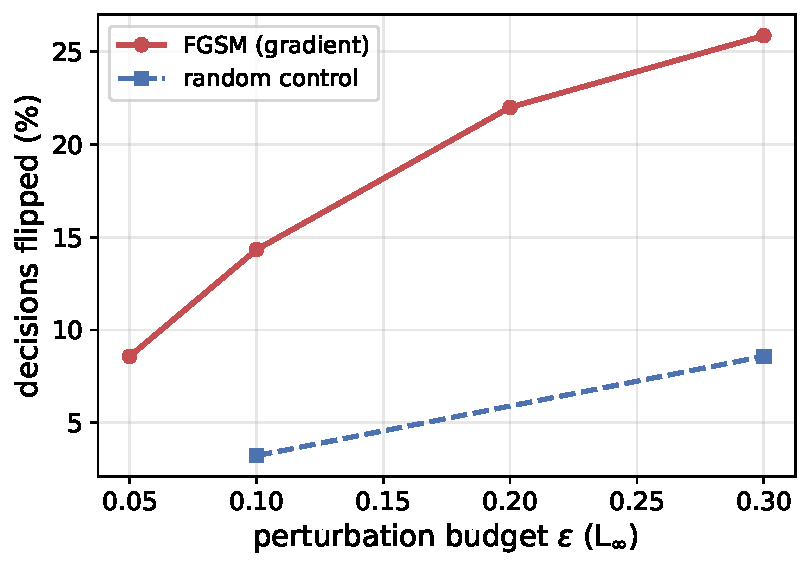
\includegraphics[width=0.9\linewidth]{T1_flip_vs_epsilon.pdf}
  \caption{Action-flip rate vs.\ budget $\epsilon$ (CC-Simple, $2\times$ hotspot).
  FGSM flips ${\sim}3\times$ more decisions than a budget-matched random perturbation.}
  \label{fig:flips-eps}
\end{figure}
\begin{figure}[t]\centering
  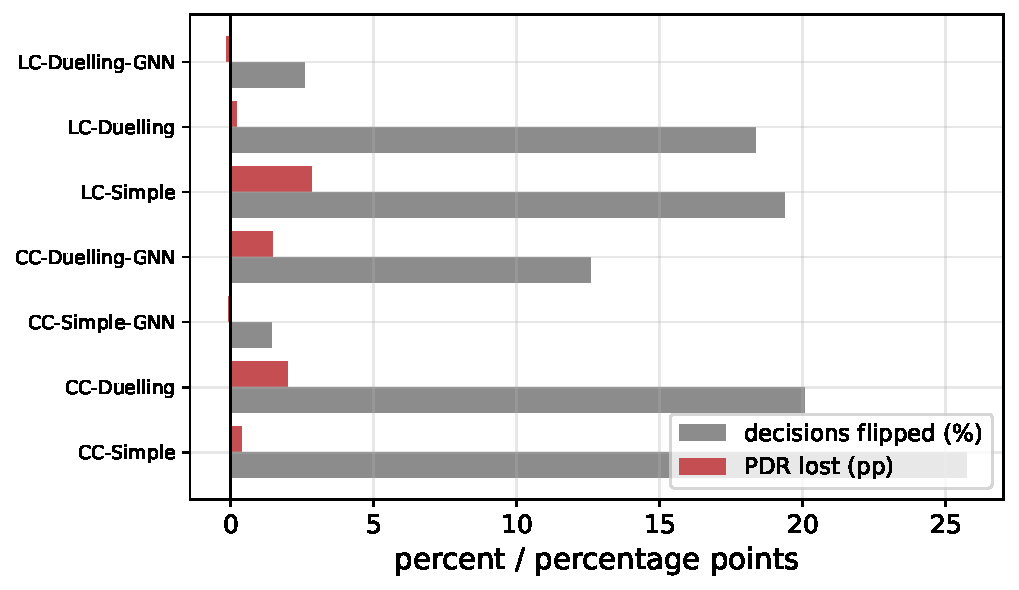
\includegraphics[width=0.9\linewidth]{T2_flips_vs_pdr_nominal.pdf}
  \caption{Decisions changed vs.\ delivery lost, seven variants, $\epsilon{=}0.3$.
  Many decisions flip; almost no packets are lost.}
  \label{fig:flips-pdr}
\end{figure}
\begin{figure}[t]\centering
  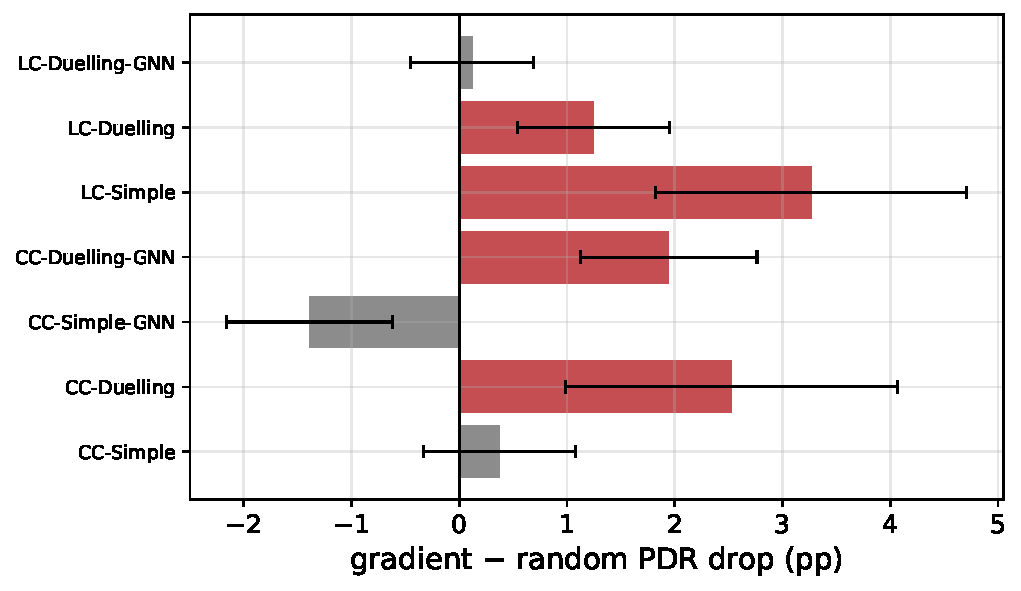
\includegraphics[width=0.9\linewidth]{T3_adversarial_gap_by_variant.pdf}
  \caption{Adversarial-specific effect (gradient $-$ random drop), paired $95\%$ CI.
  Red bars exclude zero (a real targeted signal); grey include zero.}
  \label{fig:gap}
\end{figure}
\begin{figure}[t]\centering
  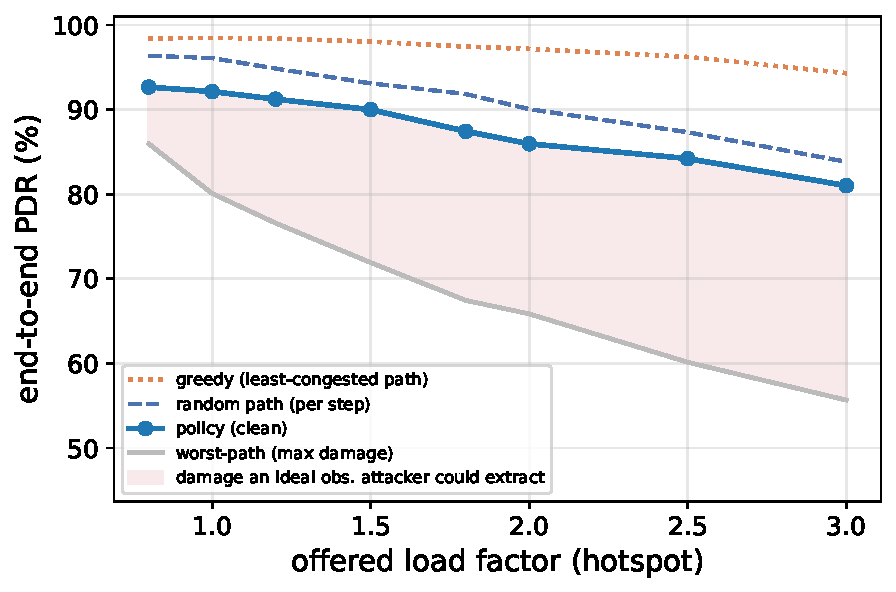
\includegraphics[width=0.9\linewidth]{T7_damage_ceiling_contrast.pdf}
  \caption{Damage ceiling vs.\ achieved damage across load. FGSM extracts almost none
  of the delivery an ideal decision-steering attacker could destroy (shaded band).}
  \label{fig:ceiling}
\end{figure}
\begin{figure}[t]\centering
  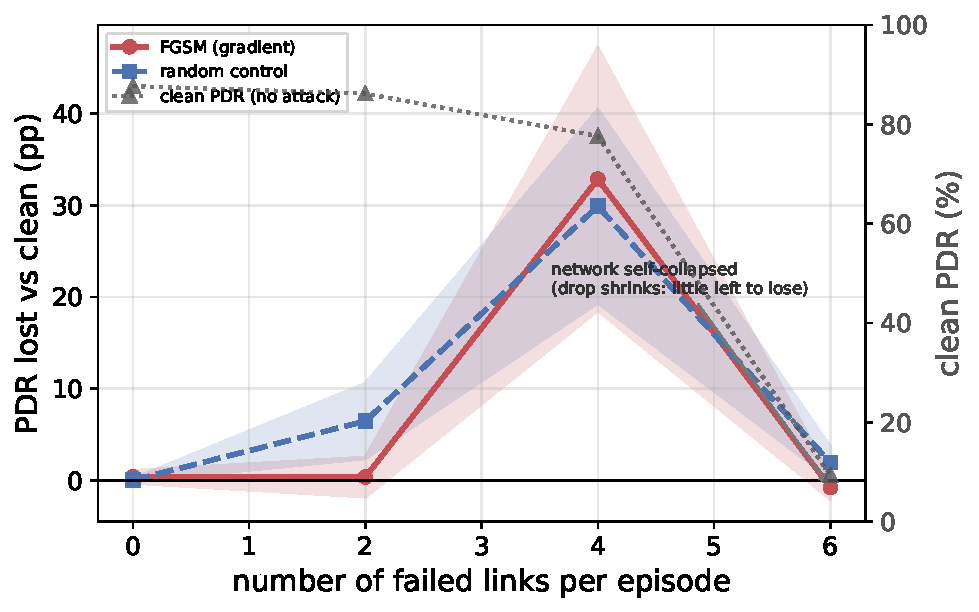
\includegraphics[width=0.9\linewidth]{T4_failure_fragility.pdf}
  \caption{Delivery drop vs.\ failed links (CC-Simple), gradient and random with paired
  CI bands; grey clean-PDR line (right axis). Random $\geq$ gradient throughout.}
  \label{fig:fragility}
\end{figure}

\section{Learned Worst-Case Adversary (Method + Protocol)}
\label{sec:learned}
The myopic result raises one question above all: is the redundancy-based robustness
\emph{fundamental}, or did FGSM simply fail to find the attack? A single-step,
per-agent gradient is myopic (it optimises the current step, not the trajectory) and
uncoordinated (it perturbs each agent independently), yet the damage ceiling is an
inherently \emph{coordinated, multi-step} outcome --- flows herded onto shared
bottlenecks over time. We therefore formulate the strongest attacker in the same threat
model: the optimal observation adversary of the state-adversarial MDP.

\subsection{SA-MDP formulation}
Fix the victim policy $\pi$. The adversary is a policy $\nu$ that, at each step, maps
the true observation $o$ to a perturbation $\delta\in\mathcal{B}_\infty(\epsilon)$; the
victim then acts on $\tilde o = \Pi(o+\delta)$, where $\Pi$ projects into the
$\epsilon$-ball and the admissible $[0,1]$ range. The adversary's reward is the
victim's per-step packet loss, $r^\text{adv}_t = L_t$, so maximising the adversary's
return minimises the victim's delivery over the trajectory. This is exactly the SA-MDP
optimal adversary of~\cite{zhang2020robust}, and unlike FGSM it optimises the
\emph{discounted trajectory} return, capturing multi-step herding that a one-step
gradient cannot.

\subsection{Training algorithm}
We train $\nu$ by DDPG against the frozen victim (Algorithm~\ref{alg:adv}): a
deterministic adversary actor emits $\delta$, a critic estimates the adversary's
action value, and updates ascend the victim's packet loss. The victim's weights are
never updated. The algorithm is instantiated in the released scaffold
(\texttt{src/attack\_framework/learned\_adversary.py}, driver
\texttt{tools/train\_adversary.py}); the trained adversary exposes the same interface
as the FGSM attacker, so it is scored by the identical paired protocol of
Section~\ref{sec:method}.

\begin{algorithm}[t]
\caption{Learned observation adversary (SA-MDP, DDPG)}
\label{alg:adv}
\begin{algorithmic}[1]
\State \textbf{Input:} frozen victim $\pi$, env, budget $\epsilon$
\State init adversary actor $\nu_\theta$, critic $Q_\phi$, targets, replay $\mathcal{R}$
\For{each episode}
  \State reset env; observe $o$
  \For{each step}
    \State $\delta \gets \operatorname{clip}(\nu_\theta(o)+\text{noise},-1,1)\cdot\epsilon$
    \State $\tilde o \gets \Pi_{\epsilon,[0,1]}(o+\delta)$ \Comment{project to ball + domain}
    \State $a \gets \pi(\tilde o)$; step env; observe $o'$, loss $L$
    \State store $(o,\delta,L,o')$ in $\mathcal{R}$
    \State sample batch; update $Q_\phi$ (TD on $L$), $\nu_\theta$ (ascend $Q$)
    \State soft-update targets; $o\gets o'$
  \EndFor
\EndFor
\end{algorithmic}
\end{algorithm}

\subsection{Structure-aware variants}
\textbf{Coordinated (multi-agent).} A single adversary emits a \emph{joint}
perturbation over several compromised provider edges, with a critic conditioned on the
global link state, so it can push multiple flows onto one shared surviving link ---
the mechanism the per-agent gradient cannot express, and the one most likely to reach
the ceiling. \textbf{Strategically-timed.} Given an $L_0$ budget (a cap on the fraction
of steps attacked), the adversary spends perturbations only at high-leverage moments
--- congestion onset, or immediately after a failure when redundancy is thin --- gated
by a critical-state score. Both are stubbed as extension points in the scaffold.

\subsection{Evaluation protocol and hypotheses}
The learned adversary is evaluated exactly as FGSM: paired clean/attacked episodes,
action-flip and delivery-drop, adversarial-specific gap vs.\ the random control, and
achieved damage vs.\ the ceiling, at nominal load and across the failure sweep, for all
seven variants. Two outcomes are scientifically decisive:
\begin{itemize}
  \item \textbf{H1 (robustness is fundamental).} If the learned/coordinated/timed
  adversary still extracts a small fraction of the damage ceiling at nominal load, then
  redundancy is a genuine structural defence and the myopic result was not an artefact
  of a weak attack --- the strong, publishable negative.
  \item \textbf{H2 (myopia hid a vulnerability).} If the learned adversary extracts
  substantially more than FGSM --- especially the coordinated variant approaching the
  ceiling --- then observation attacks \emph{can} degrade the policy once they optimise
  trajectories and coordinate, and the defence recommendation shifts from ``redundancy
  suffices'' to ``telemetry integrity is required.''
\end{itemize}

\subsection{Results: the stronger attacker does not extract more}
\label{sec:learned-results}
Twenty-eight adversaries were trained, one per combination of victim variant, attack
scope (independent or coordinated) and domain constraint, and each was evaluated at four
timing budgets and without one, giving 140 configurations. All runs use $\epsilon{=}0.30$
with every agent compromised, the $2\times$ hotspot regime and no link failures, scored
on 30 paired episodes against an unperturbed arm and a random control drawn from the same
admissible set. Because the earlier study clamped only the first four observation features
after projection, results are reported under that same \emph{FGSM-parity} constraint and,
separately, under a stricter clamp in which every feature is re-projected; only the former
is directly comparable with the baseline.

The comparison is made on the 15 episodes the two evaluations share, and it is decisive in
the negative. \textbf{The learned adversary did more total damage than FGSM in one of the
70 comparable configurations} --- the ungated independent attack on \texttt{LC-Simple}, by
$2.21$\,pp. Everywhere else it matched the baseline or fell short of it, significantly so
on four variants at every timing budget. Part of that shortfall is by construction, since a
gated attack acts on 10--25\% of steps while FGSM acts on all of them; normalising by the
realised attack rate, the learned attack does buy more damage \emph{per attacked step} on
individual variants, but this never carries through to more damage in total.

Coordination changes which victims are harmed rather than how much: under the parity clamp
it significantly increased the damage to \texttt{LC-Duelling} and \texttt{CC-Duelling} while
\emph{reducing} it on \texttt{LC-Simple}, the variant the independent attack harmed most,
and under the stricter clamp the pattern reversed again. No single property of the victim
predicts the direction. The timing gate realises its budget accurately and fires on
genuinely congested states, and on some variants concentrating the budget buys up to
$2.6\times$ the damage per attacked step; it does not buy more damage overall, and for
almost every attackable victim the ungated attack remains the most damaging.

Three findings hold across the evaluation. The fraction of routing decisions an attack
changes does not predict the damage it does: attacks that changed 13--15\% of decisions
produced gaps spanning more than seven percentage points, which is the decision--outcome
split of Section~\ref{sec:myopic} appearing again inside a single attacker family.
\texttt{CC-Simple-GNN} and \texttt{LC-Duelling-GNN} were not harmed by any attack in any
setting, for different reasons --- the first barely changes its routing under perturbation
at all, the second changes it and delivers regardless --- yet GNN encoding is not
protective in itself, since \texttt{CC-Duelling-GNN} suffered the largest gap of the
stricter-clamp independent attack. And one trained adversary steered \texttt{LC-Duelling}
to deliver \emph{more} than it did unattacked, which shows a learned attacker can fail to
find damage that exists.

This favours \textbf{H1} in its weaker form. An attacker whose policy class contains FGSM's
per-step rule, and which can additionally coordinate across agents and choose when to act,
ends up doing about as much damage as a single gradient step. That is what one expects of a
controller whose redundancy absorbs decision-level perturbation, and not what one expects if
the myopic result had merely reflected a weak attack. It does not, however, establish
robustness, for two reasons that Section~\ref{sec:threats-to-validity} develops: the effects
are of the order of one or two percentage points on a delivery ratio near $77\%$, comparable
to what an undirected perturbation of the same size moves; and each configuration was
trained once, so the reported intervals capture variation between evaluation episodes but
not between training runs. What the evidence supports is the weaker statement that no attack
in this family, as trained here, did substantial damage to these controllers.

\section{Threats to Validity}
\label{sec:threats-to-validity}
The claims this study can support are bounded by four things, and we state them because
several are large relative to the effects reported.

\textbf{Training-run variation.}
\label{sec:seeds}
Every number in Sections~\ref{sec:myopic} and~\ref{sec:learned-results} describes particular
trained networks. On the victim side we retrained the four non-GNN variants under three
independent seeds and re-ran the nominal probe on each: the adversarial-specific gap moves
by more between seeds of one architecture than between architectures, so per-variant
comparisons are not attributable to design (Section~\ref{sec:myopic}). The three GNN variants
were trained once and are reported as such. On the attacker side each of the 28 learned
adversaries was likewise trained once, so the intervals of
Section~\ref{sec:learned-results} cover variation between evaluation episodes and not
between training runs; a significant gap there shows that \emph{the adversary that was
trained} beat its control on those episodes, not that the configuration would do so
reliably if trained again. Comparisons between separately trained adversaries --- the
effect of coordination, the effect of the domain clamp, the comparison with FGSM --- are
the most exposed to this, and the aggregate conclusion, that no attacker in the family
extracts a large share of the ceiling, is the least exposed.

\textbf{Effect sizes against uncontrolled variation.} Almost every reported difference is
one or two percentage points on a delivery ratio near $77\%$. A perturbation of the same
magnitude with no adversarial direction moves delivery by a comparable amount and in either
direction, which is why the budget-matched random control, not the clean arm, is the
reference throughout. A paired interval can resolve a difference this small between two arms
on the same episodes, but resolving a difference is not the same as attributing it.

\textbf{Sampling.} All evaluations draw on a single traffic seed, so variation between
traffic patterns is sampled only by the episodes within it. Several hundred confidence
intervals are reported at the 95\% level without correction for multiple comparisons, so a
few cells can be expected to exclude zero by chance; the conclusions rest on patterns that
hold across conditions rather than on individual cells.

\textbf{Measurement.} The action-flip rate overstates an attack's reach. Candidate paths are
$K$-shortest routes deduplicated by first hop, and pairs with fewer than $K$ genuinely
distinct routes are padded by repeating the shortest one, so a flip between two padded slots
changes the decision and routes the packet identically. Measured directly, $8$--$22\%$ of
flips are vacuous in this sense, and the share differs by variant, so flip rates are not
strictly comparable across architectures. This reinforces rather than weakens the central
finding: the decision-level effect of these attacks is smaller still than the raw rates
suggest, while the delivery effect is unchanged.

\textbf{Scope.} One topology, one stressed traffic regime, one perturbation budget for the
learned attacker, and a simulator rather than a testbed. The redundancy mechanism we
advance is a property of a well-provisioned service-provider graph with $K$ disjoint-ish
paths per destination; we do not claim it holds where path diversity is thin.

\section{Discussion}
\label{sec:discussion}
The organising lesson is the split between changing \emph{decisions} and changing
\emph{outcomes}. On a redundant transport topology these come apart: a competent
decision-level attack (FGSM flips a quarter of choices, $3\times$ noise) leaves
delivery almost untouched because $K$-path redundancy reroutes the moved flows. The
random control keeps the interpretation honest --- the failure-regime collapse is noise,
not adversary --- and the damage ceiling quantifies how little of the available harm is
reached. Whether this robustness is fundamental is exactly what the learned adversary
tests; the paper is structured so that either answer (H1 or H2) is a result. For
operators the guidance is already actionable under the completed results: adversarial
training against FGSM would defend a boundary redundancy already protects, while doing
nothing for the failure regime, where the threat is undirected noise --- so investment
belongs in telemetry integrity and fast reconvergence. The learned-adversary study will
sharpen this into a threat-model-complete recommendation.

\section{Conclusion}
\label{sec:conclusion}
We framed observation-attack robustness of multi-agent routing around a progression of
attackers and two references (a random control and a damage ceiling), and showed that a
myopic gradient attack changes many decisions but almost no outcomes on a redundant SP
topology, with the failure-regime fragility exposed as noise rather than adversary. The
decisive next step --- a learned worst-case adversary, coordinated and timed --- is
formulated here and released as an open scaffold, so that the question of whether
redundancy is a genuine adversarial defence can be settled rather than assumed.

\begin{thebibliography}{1}
\small
\bibitem{companion} P.~Amaral and D.~Raimundo, ``Centralised or Local Critic?
Mechanism-Grounded Selection of MADDPG Architectures for Adaptive Routing,'' companion
manuscript, 2026.
\bibitem{goodfellow2015} I.~J. Goodfellow, J.~Shlens, and C.~Szegedy, ``Explaining and
Harnessing Adversarial Examples,'' in \emph{Proc. ICLR}, 2015.
\bibitem{huang2017adversarial} S.~Huang \emph{et al.}, ``Adversarial Attacks on Neural
Network Policies,'' in \emph{Proc. ICLR Workshop}, 2017.
\bibitem{lin2017tactics} Y.-C. Lin \emph{et al.}, ``Tactics of Adversarial Attack on
Deep Reinforcement Learning Agents,'' in \emph{Proc. IJCAI}, 2017.
\bibitem{sun2020stealthy} J.~Sun \emph{et al.}, ``Stealthy and Efficient Adversarial
Attacks against Deep Reinforcement Learning,'' in \emph{Proc. AAAI}, 2020.
\bibitem{zhang2020robust} H.~Zhang \emph{et al.}, ``Robust Deep Reinforcement Learning
against Adversarial Perturbations on State Observations,'' in \emph{Proc. NeurIPS},
2020.
\bibitem{zhang2021robust} H.~Zhang \emph{et al.}, ``Robust Reinforcement Learning on
State Observations with Learned Optimal Adversary,'' in \emph{Proc. ICLR}, 2021.
\bibitem{survey2025} Anon., ``Enhancing Security in Deep Reinforcement Learning: A
Survey on Adversarial Attacks and Defenses,'' \emph{arXiv:2510.20314}, 2025.
\bibitem{camouflage2024} Anon., ``Camouflage Adversarial Attacks on Multiple Agent
Systems,'' \emph{arXiv:2401.17405}, 2024.
\bibitem{wolfpack2025} Anon., ``Wolfpack Adversarial Attack for Robust Multi-Agent
Reinforcement Learning,'' \emph{arXiv:2502.02844}, 2025.
\bibitem{packetlevel2024} Anon., ``Learning Sub-Second Routing Optimization in Computer
Networks requires Packet-Level Dynamics,'' \emph{arXiv:2410.10377}, 2024.
\end{thebibliography}
\end{document}
